\documentclass[12pt, twoside,openright,a4paper,papersize,uplatex,dvipdfmx, report]{jsbook}
% uplatex オプションを指定し、ユニコード対応に。ただだし、uplatex でコンパイルすること。

% 修論本体と表紙で共通で必要となる設定
% jsbookで余白が広すぎるのを直す
% 参照 https://oku.edu.mie-u.ac.jp/~okumura/jsclasses/
\setlength{\textwidth}{\fullwidth}
\setlength{\evensidemargin}{\oddsidemargin}
\addtolength{\textwidth}{-5truemm}
\addtolength{\oddsidemargin}{5truemm}

% 同梱の ISEE 用の表紙テンプレ
\usepackage{thesis_cover}

% OTF フォントを使えるようにし、複数のウェイトも使用可能にする。
% これがないと、Mac のヒラギノ環境で使われる角ゴが太すぎてみっともない。
\usepackage[deluxe]{otf}
% OT1→T1に変更し、ウムラウトなどを PDF 出力で合成文字ではなくす
\usepackage[T1]{fontenc}
% uplatex の場合に必要な処理 
\usepackage[utf8]{inputenc} % エンコーディングが UTF8 であることを明示する。
\usepackage[prefernoncjk]{pxcjkcat} % アクセントつきラテン文字を欧文扱いにする
% Helvetica と Times を sf と rm のそれぞれで使う。
% default だとバランスが悪いので、日本語に合わせて文字の大きさを調整する。
\usepackage[scaled=1.05,helvratio=0.95]{newtxtext}
% 色
\usepackage[dvipdfmx]{color}
% 行番号を表示する。
\usepackage{lineno}

% latexdiff
% 実際の修論には入れる必要なし
%DIF PREAMBLE EXTENSION ADDED BY LATEXDIFF
%DIF UNDERLINE PREAMBLE %DIF PREAMBLE
\RequirePackage[normalem]{ulem} %DIF PREAMBLE
\RequirePackage{color}\definecolor{RED}{rgb}{1,0,0}\definecolor{BLUE}{rgb}{0,0,1} %DIF PREAMBLE
\providecommand{\DIFadd}[1]{{\protect\color{blue}\uwave{#1}}} %DIF PREAMBLE
\providecommand{\DIFdel}[1]{{\protect\color{red}\sout{#1}}}                      %DIF PREAMBLE
%DIF SAFE PREAMBLE %DIF PREAMBLE
\providecommand{\DIFaddbegin}{} %DIF PREAMBLE
\providecommand{\DIFaddend}{} %DIF PREAMBLE
\providecommand{\DIFdelbegin}{} %DIF PREAMBLE
\providecommand{\DIFdelend}{} %DIF PREAMBLE
%DIF FLOATSAFE PREAMBLE %DIF PREAMBLE
\providecommand{\DIFaddFL}[1]{\DIFadd{#1}} %DIF PREAMBLE
\providecommand{\DIFdelFL}[1]{\DIFdel{#1}} %DIF PREAMBLE
\providecommand{\DIFaddbeginFL}{} %DIF PREAMBLE
\providecommand{\DIFaddendFL}{} %DIF PREAMBLE
\providecommand{\DIFdelbeginFL}{} %DIF PREAMBLE
\providecommand{\DIFdelendFL}{} %DIF PREAMBLE
%DIF END PREAMBLE EXTENSION ADDED BY LATEXDIFF


%% 以下追加したpackage
% 画像の取り扱いに必要
\usepackage{graphicx}
% 数式の機能を拡張
\usepackage{amsmath}
\usepackage{bm}
\usepackage{upgreek}
\usepackage{newtxmath,newtxtext}
% コードを表示
\usepackage{listings}
\lstset{
    %プログラム言語(複数の言語に対応,C,C++も可)
    language = Python,
    %背景色と透過度
    backgroundcolor={\color[gray]{.98}},
    %枠外に行った時の自動改行
    breaklines = true,
    %自動改行後のインデント量(デフォルトでは20[pt])	
    breakindent = 10pt,
    %標準の書体
    basicstyle = \ttfamily\scriptsize,
    %コメントの書体
    commentstyle = {\itshape \color[cmyk]{1,0.4,1,0}},
    %関数名等の色の設定
    classoffset = 0,
    %キーワード(int, ifなど)の書体
    keywordstyle = {\bfseries \color[cmyk]{0,1,0,0}},
    %表示する文字の書体
    stringstyle = {\ttfamily \color[rgb]{0,0,1}},
    %枠 "t"は上に線を記載, "T"は上に二重線を記載
    %他オプション:leftline,topline,bottomline,lines,single,shadowbox
    frame = tbrl,
    %frameまでの間隔(行番号とプログラムの間)
    framesep = 5pt,
    %行番号の位置
    numbers = left,
    %行番号の間隔
    stepnumber = 1,
    %行番号の書体
    numberstyle = \tiny,
    %タブの大きさ
    tabsize = 4,
    %キャプションの場所("tb"ならば上下両方に記載)
    captionpos = t
}
% 複数引用
\usepackage{cite}
% jecon.bstを使う時に必要.それ以外ではエラーが出るのでコメントアウトする.
%\usepackage{natbib}
% 複数図を並べる時のcaption
\usepackage{subcaption}
\usepackage{here}
% 表関連
\usepackage{booktabs}
% 表でセルを複数列で結合する
\usepackage{multicol}
\usepackage{multirow}
% PDF 内で外部リンクや文書内リンクを生成したい場合に使う(好みによる)
\usepackage[dvipdfmx, hidelinks]{hyperref}
\usepackage{url}
% 複数行コメント
\usepackage{comment}
% 番号付き箇条書きのオプション利用
\usepackage{enumerate}
% renewcommandなどはここに
\usepackage{mymacros}
% 目次でsubsectionまで表示
\setcounter{tocdepth}{2}



% 画像の取り扱いに必要
\usepackage{graphicx}
% 数式の機能を拡張
\usepackage{amsmath}
\usepackage{bm}
\usepackage{upgreek}
\usepackage{newtxmath,newtxtext}
% 複数引用
\usepackage{cite}
%\usepackage{natbib}
% 複数図を並べる時のcaption
\usepackage{subcaption}
\usepackage{here}
% 表関連
\usepackage{booktabs}
% 表でセルを複数列で結合する
\usepackage{multicol}
\usepackage{multirow}
% 行番号を表示する。添削時のみに使い、事務提出版ではコメントアウトする
%\usepackage{lineno}
%\linenumbers
% PDF 内で外部リンクや文書内リンクを生成したい場合に使う(好みによる)
\usepackage[dvipdfmx, hidelinks]{hyperref}
\usepackage{url}
% renewcommandなどはここに
\usepackage{mymacro}
% 目次でsubsectionまで表示
\setcounter{tocdepth}{2}
% 複数行コメント
\usepackage{comment}


% 氏名などの情報が入っているファイル。各自で編集。
%\title{機械学習を用いたパーソナルロボットハンドの開発\\~上肢機能障害者の支援を目指して〜} % 論文題目
\date{2020年1月30日} % 日付(入れたくなければ空欄)
\seireki{2020} % 年度
\StudentIdNumber{37-186508} % 学籍番号
\author{山田敦史} % 氏名
\seifuku{} % 正本か副本か(このファイルでは変更する必要なし)
% \labname{宇宙線物理学研究室} %
\supervisor{小野寺宏 特任教授} % 指導教員
\cosupervisor{染谷隆夫 教授} % 副指導教員


\begin{document}
% 式番号,図番号,表番号を章ごとの連番にする
\numberwithin{equation}{chapter}
\numberwithin{figure}{chapter}
\numberwithin{table}{chapter}


\frontmatter

%\maketitle

% これを入れることでページ番号が表示されない。
%\thispagestyle{empty}

% abstract 環境は jsbook では「概要」と表示してくれないため、手動で表示させる。
% 参照 http://oku.edu.mie-u.ac.jp/tex/mod/forum/discuss.php?d=2121
\begin{center}
  {\large \sf 概要}
\end{center}

% 170字以内
上肢機能障害者の生活を支援するロボットとして携帯可能な小型自律ロボット,パーソナルロボットハンドを開発した.試作1号機ではスマートフォンを用いたローカル演算に夜強化学習によって,特定の色の物体のピックアップに成功した.試作2号機では深層学習を用いて対象物を識別し,指定した物体に接近・把持し,元の場所へ持ち帰ることに成功した.
% (163)


% 最近の義手は主に筋電図(EMG)によって駆動される。しかしEMG駆動は汗に弱いという問題があり、トレーニングが必要である。一方、最近では、より人間の生活に密着したロボット、例えば、整体ロボットが開発されている。そこで本研究では、筋電図制御ではなく強化学習を用いた、人間の手とは独立したロボットハンドを提案する。今回、スマートフォンを使って特定の色の物体を拾うことに成功した。


\tableofcontents
\listoffigures
\listoftables

\mainmatter

% include を使うことで、別ファイルに分割することができます。
\chapter{序論}
\label{chap_intro}

\section{研究背景}
ロボティクス技術の向上とともに,様々な分野でロボットが活躍している.特に,医療や福祉といった人間の生活環境下で作業可能なパーソナルロボットの需要の増加は顕著である.しかし,人の生活環境下において完全に自律して動作及び人の補助ができるロボットの実現は困難な状況にある.なぜならば,ロボットが自律行動を行うためには物体や人物の認識,自己位置の認識,そして認識に基づく判断を人の生活環境下で行わなければならないからである.

パーソナルロボットとしてMobile manipulatorの開発が行われている.Mobile Manipulatorは工場に限定されて使用されているが,これを家庭内でも使用できるように軽く,そして小さくすることで衝突リスクを削減する試みがされている.2018年には,Preferred Networksは室内に散らかった家庭用品を片付けるロボットシステムを発表した\cite{お片づけロボット}.部屋の全自動片付けは従来のロボットシステムでは実現困難であったが,近年の深層学習の発展によって初めて実用的なレベルとなった.物をつかむ,物を置く,動作計画を立てる,人の指示に対応するなど,ロボットが人間の生活空間で仕事をするために必要な物体認識・ロボット制御・音声言語理解技術に最先端の深層学習を用いた結果,ロボットが高速・高精度に動作できるようになった.

一方,医療分野におけるロボットで一番身近なものと言えば義手である.義手には装飾用義手や能動義手,作業用義手などがあるが,現在主流の筋電電動義手(筋電義手)は,使用者が筋肉を動かすことで筋電位を読み取り直感的な操作を可能にする.しかし,筋電位を用いた義手には訓練が必要でリハビリテーション施設で行う必要があるが,その施設が極めて少ない\cite{リハビリテーション}.また筋電位が上手く出せない患者や,腕そのものはあるが麻痺して動かせない患者に対しては使用できない.さらに非侵襲的な筋電義手では入力信号が限られる.自由度の高い動作を可能にすると重量が大きくなり,使用者の負担が大きくなってしまう.
実際に筆者が茨城県立大学付属病院リハビリテーション科に見学に行った際,義手使用患者へヒアリングをした.
当患者は普段は能動義手を使用しており,リハビリの際に筋電義手も使用している.半年のリハビリでペンを掴むことまでできたという状況である.
筋電義手の使い心地について聞いたところ,「筋電義手は重い」「(筋電が)ちゃんと伝わっているかわからない」「把持力の制御が難しく,落とすこともよくある」とあまりポジティブな感想はなかった.
以上のような課題があるため装着者のニーズを満たす義手がなく,あまり普及していないのが現状である.


\section{関連研究}
ここではロボット開発の研究について紹介する.

TOYOTAはHuman Support Robot(HSR)を開発した\cite{HSR}.



机に置いて使うもの
Basic research of upper limb work support system “My Cybernic Robot Arm” for hemiplegic persons


強化学習で制御
教師ありで制御

推論時の計算リソースが必要となる.
cloudリソースを使用する方法がある.これはcloudとのインターフェースを有しているデバイスであれば演算性能は低くても推論が可能となり,スマートフォンやノートPC,ラズパイと言った小さなデバイスを使用することができる.しかし常時インターネットに接続している必要があるため,災害時に使用できなくなるという問題がある.
そこで,cloudではなくlocalで(Edgeで)推論を行うエッジデバイスを使用することがある.

\section{研究目的}
携帯できる生活支援ロボットの開発
タスク:机の上に限定した,ピックアップ
今回はlocalで(Edgeで)処理することにする


 % 背景
\chapter{深層学習による病理画像の診断支援}
\label{chap_review}

病理画像をデジタルで保存することが始まったのは数十年前になる.これによって遠隔地でも診断することができるようになったり,情報を共有することができるようになり,複数の医師で診断しミスを防止するセカンド・オピニオンが容易になった.計算機科学の分野の側面ではデータを収集することができるようになり,研究が盛んに行われることになった.その後は,様々な病理データでより改良されたアルゴリズムの提案が行われている.

細胞組織の形態を観察するための病理染色ではヘマトキシリン・エオジン染色(HE染色)が一般的に用いられる.細胞核を青紫色に染色し,細胞質をピンク色に染色する.正常から異常に変化していくと,細胞核が過度に増殖したり,細胞質の形が崩れたりすることで,その特徴を機械学習によって精度よく検出するための研究が行われている.

これまでは,核の形やテキスチャーからパターンマッチングなどの画像処理によって腫瘍を検出する研究されてきたが,近年になって画像処理に大きなブレークスルーが起きたことをきっかけに,新しい手法で解析するようになってきた.そのブレークスルーがディープラーニングである.



\section{ニューラルネットワーク}
人間の脳にはニューロンと呼ばれる神経細胞が1000億個以上あり,それぞれが複数のニューロンと電気信号で情報を伝達している.また脳には電気信号を受け渡すシナプスという場所がある.ニューロンとシナプスで行われる演算を模倣したアルゴリズムを作ることができれば人間のような思考や認識をコンピュータを使って再現できると考えた.そのアルゴリズムがニューラルネットワークである.

\subsection{多層パーセプトロン}
ニューラルネットワークは入力層,出力層,隠れ層から構成され,層と層の間にはニューロン同士のつながりの強さを示す重みがある.非線形問題を扱うために 1986 年 Rumelhart によって考案されたのが,パーセプトロンを複数つなぎ合わせ入力と出力以外に隠れた層を持つ多層パーセプトロン (Multi-layer perceptron: MLP) である.

ニューラルネットワークで多層パーセプトロンの層を全結合(fully connected: FC) 層とも呼ぶ.Figure 3.1 における丸や矢印はそれぞれノード (またはニューロン) と重み (または結合) と呼び,ともに数値である.例えば画像を分類しようと思えば,各ピクセルの画素数を各ノードに入力する (28×28pix のグレースケール画像であれば 784 個のノードが必要).データが入力層に入ってくると,その値に重みをかけ,活性化関数と呼ばれる関数を通し結果を出力する.これを繰り返し出力層に書き出す.各層の重みの値によって出力結果は異なってくる.出力層のノードは区別したいクラス数分用意し,各ノードの出力値が各クラスに属している確率を表す.学習については誤差逆伝播法を利用する.ニューラルネットワークの出力値と正解データとの比較をした時に,どれだけ正解から離れているかを評価する損失関数 (Loss) を使って,損失関数が小さくなるようにノード間の重みを勾配降下法によって更新する.

\subsection{畳み込みニューラルネットワーク}
畳み込みニューラルネットワーク (ConvolutionalNeural Network: CNN) は,1998 年には既に LeNetと呼ばれるネットワークで実装されていた [3].従来の画像認識では,画像から特徴を抽出し,それをニューラルネットワークにかけるいわゆる特徴量設計が必要で,ここをいかにうまく設計するかがポイントであったが,CNN は特徴量設計から識別までを end-to-end で行うことがきることが最大の強みである.人間が物体を認識することをコンピュータにも計算させるには,画像の特徴的な部分を切り分けて数値化させる必要がある.例えば,カラー画像の場合,RGB の 3 色 (3 チャンネル)を組み合わせた画像で認識をしている.このようなフィルターの畳み込み計算を行うと,フィルターごとに異なった画像の特徴を抽出して数値化する.これが畳み込み (convolution) である.その後,画像のサイズを小さくしてコンピュータが計算コストを減らし,微小な変化に対してロバストになる仕組みしてプーリングという方法を用いる.学習には MLPと同様に誤差逆伝播法を用いる.


\subsection{再帰的ニューラルネットワーク}
再帰的ニューラルネットワーク(Recurrent Neural Network: RNN)
Long-short term memory(LSTM)


\begin{figure}[h]
\centering
\includegraphics[width=0.7\linewidth]{fig/lstm.png}
\caption{}
\label{fig:LSTM}
\end{figure}

\begin{align}\label{eq:LSTM}
  i_t & = \sigma(W_{xi} x_t + W_{hi} h_{t-1} + W_{ci} c_{t-1} + b_i) \\
  f_t & = \sigma(W_{xf} x_t + W_{hf} h_{t-1} + W_{cf} c_{t-1} + b_f ) \\
  c_t & = f_t c_{t-1} + i_t tanh(W_{xc} x_t + W_{hc} h_{t-1} + b_c) \\
  o_t & = \sigma(W_{xo} x_t + W_{ho} h_{t-1} + W_{co} c_t + b_o) \\
  h_t & = o_t tanh(c_t) 
\end{align}

ここで$\sigma$はシグモイド関数であり,次の式で定義される.
\begin{equation}\label{eq:sigmoid}
  \sigma (x) = \dfrac{1}{1 + e^{-x}}
\end{equation}


\section{画像認識におけるディープラーニング}
Deep Learning とは Deep Neural Network(DNN)を指すことが多い.この"Deep"とは,ニューラルネットワークの層が深いことに由来している.
Figure 3.3 に画像認識タスクの精度の近年の推移を示す.これは ImageNet Large Scale Visual RecognitionChallenge (ILSVRC) と呼ばれる世界的な画像認識のコンペティションである (2010 年から始まった).カテゴリ数は 1000 クラスで,画像枚数は120 万枚の訓練データと 15 万枚のテストデータが用意されている.2011 年と 2012 年は約 10\%もの大差で AlexNet[4] が優勝している.これがディープラーニングの始まりである.AlexNet は 5 つの畳み込み層と 3 つの全結合層を持っている.2014 年には VGGNet[5] や GoogLeNet[6] が 9 割の精度を超えた.VGGNet は AlexNet(8 層) よりさらに深い構造(19 層) であり,GoogLeNet は 22 層もある.そして2015 年には ResNet[7] が人間の精度をも超える認識精度を達成した.ResNet は GoogLeNet よりもさらに深く 152 層もある.一般に,層を深くすることは簡単ではなく,勾配消失や過学習といった問題が起こる.CNNを複数回かけて検出を行う場合、CNNの浅い側では空間分解能はあるが抽象的な情報が少ない。深い側では意味論的な情報は取得できる(ポーズ、変形など) が空間分解能が小さいため幾何学的な情報が失われる。アーキテクチャの進化の方向は①層が深くなること ②FC層の使用を避けること又はInceptionモジュールの使用によってパラメータ数を削減すること ③ ResNetなどのショートカット接続によって学習効率をあげること事前学習・転移学習を行うことでモデルの精度を上げる取り組みがある.当然ながらこの場合事前学習のデータセットと適用データとの間に類似性があると良い。

画像処理におけるディープラーニングでは大きく3つのタスクがあり,それぞれ,クラス分類,物体検出,セグメンテーションである.以下に詳細を述べる.

\subsection*{クラス分類}
カテゴリ分けをすること

\subsection*{物体検出}
物体検出とはBounding Boxで物体の位置とその物体の種類を特定する方法である.歴史的には幾何的情報,手動特徴量,そしてそのカスケードを利用していた.その後,HOGやSIFTなど局所特徴量を抽出する方法を設計するようになったが、これは深い専門知識を必要とした.また広い範囲でオブジェクトを正確に検出する方法は、メモリ容量と処理時間に課題がある.現在はDeep Neural Networkになりデータのみから抽象的な特徴量を複数得ることができる。一般物体認識の場合は数千のカテゴリを学習してTop Error Rateが2\%以下と人間よりも認識精度が高いが,物体検出においては,今はカテゴリがせいぜい数百程度くらいまででも認識精度が人間よりも低くなってしまう.また物体検出は精度を上げるために処理に時間がかかるアルゴリズムであることが多いため,リアルタイムに物体検出を行う時は,速度と精度でトレードオフが生じてしまう.

\begin{figure}[h]
\centering
\includegraphics[width=0.7\linewidth]{fig/yolo_ssd.png}
\caption{}
\label{fig:YOLO}
\end{figure}

\subsection*{セグメンテーション}
セマンティックセグメンテーションとは,画像を画素レベルで認識することである.画像内の各画素をオブジェクトクラスに割り当てる手法である.セマンティックセグメンテーションの手法についてディープラーニング以前では,Texton Forestsや,Random Forestsに基づいた分類を行っていたが,物体検出と同様にCNNが登場してからは,高精度なセグメンテーションが実現するようになった.CNNを使ったセグメンテーションの手法で一般的に使われるようになったものがUnetである(\fig {Unet}).このUnetは文字通りUの形をしたネットワークであることが特徴で,2つのアーキテクチャーからできている.一つ目がエンコーダーのアーキテクチャーでCNNとプーリングで特徴を抽出しながら次元を削減していき,2つ目のデコーダーのアーキテクチャーで画像をセグメンテーションの結果になるように復元する.ここで問題になることが,プーリングをすることで位置情報を消してしまっているので,この位置情報を利用して画像を復元するためには,エンコーダーとデコーダーで画像サイズが同じところ同士をショートカットで接続することがUnet構造の優れている点である.

\begin{figure}[h]
\centering
\includegraphics[width=0.7\linewidth]{fig/unet.png}
\caption{}
\label{fig:Unet}
\end{figure}

\section{深層学習による3次元画像解析}
ディープラーニングを医療画像に応用するコンペティションが世界で行われているが、その半数が3D医療画像の解析になっているほど需要が高まっている。その理由は、現在解決しなくてはならない課題があるからである。まずは2次元画像と違って、処理するべきデータが大きいということである。そのため学習するパラメータをなるべく少なくする工夫がされている。また3次元画像には、動画または、ボリューム画像があるが、2次元画像とその深さ方向(動画であれば、時間方向)には異方性があることから、機械学習の方法に工夫が必要になる。今まで考案されている手法として、2DCNNを拡張した3DCNN、またCNNと時系列解析でよく用いられるLSTMを組み合わせた手法と、LSTM内部にCNNを組み込んだ手法、それらをすべて組み合わせた手法が考案されいる。LSTMの研究も盛んに行われているため、その改良モデルが数多く存在する。特に、LSTMの学習効率を上げたGRU(Gated Linear Unit)や、順方向だけでなく逆方向の時系列も計算に入れるBiLSTMが時系列解析の精度向上になっている報告がある。


\subsection{3D CNNとStacked Convolution}
2次元画像が深さ方向に連続している3次元画像の特徴を抽出するために、2次元のCNNを拡張して、3次元のカーネルを使って畳み込みを行う、3DCNNを利用した手法がある。

\begin{figure}[h]
\centering
\includegraphics[width=0.7\linewidth]{fig/3d_cnn.png}
\caption{}
\label{fig:}
\end{figure}


\begin{figure}[h]
\centering
\includegraphics[width=0.7\linewidth]{fig/stacked_conv.png}
\caption{}
\label{fig:}
\end{figure}

\subsection{LSTMとその派生系}
LSTM+2DCNNの話


\section{ディープラーニングを用いた病理画像診断}
学習した結果を評価するときに医療画像の場合は、PrecisionとRecallを識別性能の評価指数として使う。

\begin{align}
  \mathrm{Precision} & = \dfrac{\mathrm{TP}}{\mathrm{TP}+\mathrm{FP}}\\
  \mathrm{Recall} & = \dfrac{\mathrm{TP}}{\mathrm{TP}+\mathrm{FN}}
\end{align}

ここで使ったTP(True Positive)は真の結果が正である時に予測も正であるという意味であるTN(True Negative)は真の結果が正で予測が負である場合である。同様にFP(False Positive)真の結果が負で予測も負、FN(False Negative)真の結果が負で予測は正である.

2016年に行われたCAMELYON16という乳がんの転移を調べるシステムのコンペティションでは、7人の医師の成績を上回っていることが報告されてている。

また皮膚癌の種類が757種類を細かい違いまで識別するように学習する。学習方法はInception v3というネットワークを利用している。これは22層の畳み込みニューラルネットワークである。またこのネットワークは皮膚癌の識別タスクを学習する前に、ImageNetというILSVCでも使っている一般物体画像を使って事前にネットワークの重みの初期値を決めることによって、精度が向上させる。これを転移学習(Transfer Learning)と呼ばれている。


\section{教師なし学習}
機械学習の手法には、上記で説明したように、ラベルの貼られているデータセットを用いて学習することを教師あり学習と呼び、その反対で、データセットはあっても、そのデータセットの特性を示したラベルが与えられていない場合のデータセットを用いて学習することを教師なし学習と呼ぶ。

ここで教師なし学習で画像の特徴を抽出する方法としてオートエンコーダがある。画像の場合におけるオートエンコーダの手法とは、ある画像から情報を圧縮する「エンコーダ」と言われる部分と、その圧縮した情報から画像を復元する「デコーダ」の二つからなる。入力とデコーダから復元された画像が同じ画像になるようにニューラルネットワークで学習させる。この学習の結果、潜在変数は似てる画像どうしで近い値になるように変化し、この分布を見れば画像の分類を教師ラベルがなくても、学習を行うことができる。本研究では、このオートエンコーダの派生である。Variational Autoencoder(VAE)を利用した。これはオートエンコーダの「エンコーダ」と「デコーダ」は同じネットワーク構造であるが、データセットの潜在変数の分布が、正規分布になるような制約を加えて学習を行う手法である。こうすることでAutoencoderの潜在変数では分布の距離に意味なかったが、Variational Autoencoderでは正規分布に埋め込まれるため、画像の類似度を分布が表現することができるところが特徴である。Variational Autoencoderをまずは、2Dの画像に対して分布が正常と腫瘍の画像で変化するのかを確認した。さらに3次元画像でも解析することで3DCNNを用いて画像をエンコーダのネットワークを作り、潜在変数の空間を作ることで3次元画像特有の情報を抽出することができ、2次元画像だけでは判断できない、血管構造の乱れなどが認識できるようになると考えられる。

\section{半教師あり学習}
弱教師あり学習とも呼ばれる.

 % 原理
\chapter{ロボットハンド開発に向けた要素技術}
\label{chap_experiment}


\section{強化学習による移動制御}


\section{物理シミュレーション}


\section{ARマーカーを用いた自己位置認識}


\section{インスタンスセグメンテーション}

 % 実験手法

\chapter{結果}\label{chap_result}
%loss,accのグラフは全て.
%前処理を行った場合は,その画像の一例も載せる
%モデルの画像(appendixの方がいいかもしれないです)
%各sectionで異なる場合は各sectionで載せましょう
%なるべくpdfで保存しましょう

\section{古典的な画像処理手法による識別精度評価}
%楕円検出の塗った画像
%円検出の画像
\begin{figure}[H]
	\centering
	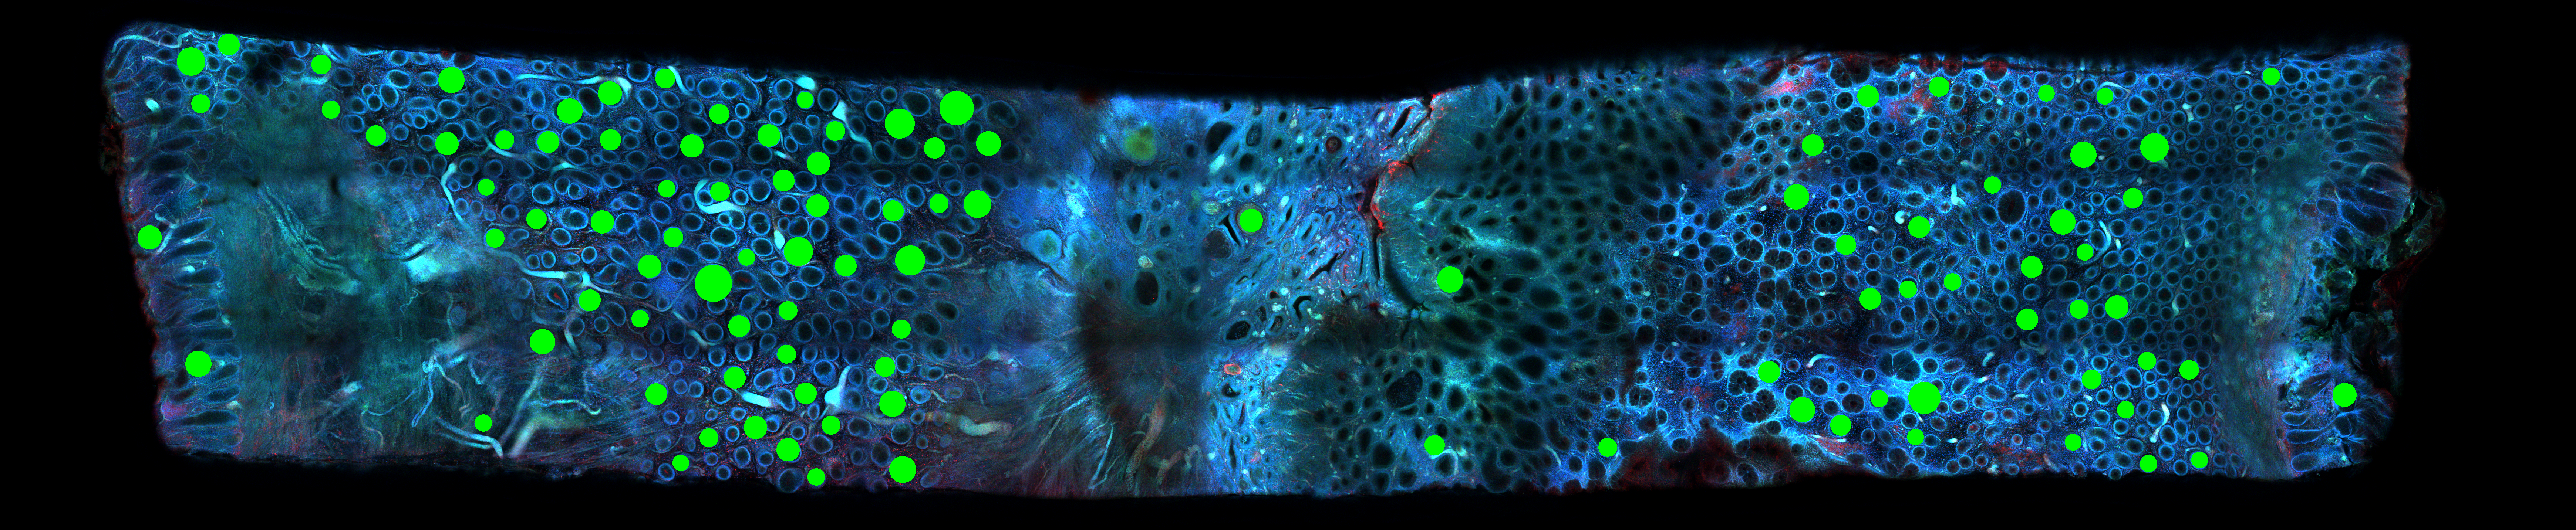
\includegraphics[width=0.7\linewidth]{fig/circle_detection}
	\caption{Detection of circle.}
	\label{fig:circle_detection}
\end{figure}

\begin{figure}[H]
	\centering
	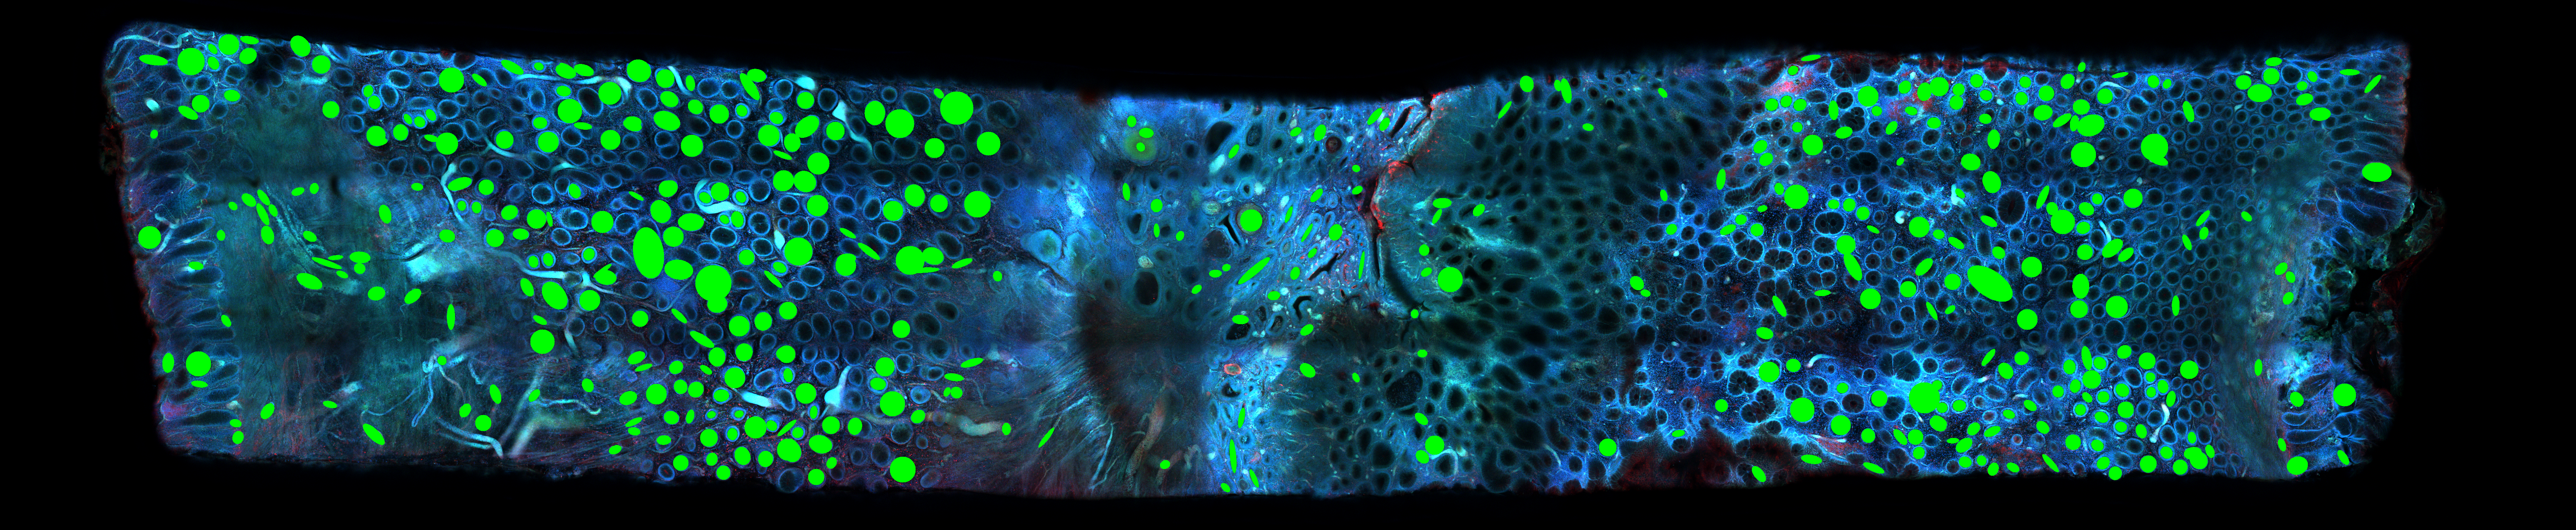
\includegraphics[width=0.7\linewidth]{fig/eclips_detection}
	\caption{Detection of ellipse}
	\label{fig:ellipse_detection}
\end{figure}

\fig{circle_detection}が円検出を利用して正常の構造を検出した結果である.緑色の円の部分が円検出された領域を示している.
真円にフィッティングしているので綺麗な円構造のみの検出となり,正常でも検出できていない部分が多くなっている.全体的に,正常領域で円検出が多く行われ,腫瘍領域では,円検出結果が少なくなる結果となったが,腫瘍部分も円検出されている部分が一部ある.

楕円検出を行った結果は\fig{ellipse_detection}で円検出よりも正常領域の検出が増えた.楕円検出がされた領域の多いところほど正常の領域で,楕円検出が少ない領域が腫瘍であるという傾向を捉えることができた.古典的な画像処理の利点は,画像検出の理由が説明できることである.このような円検出や楕円検出であれば,円形度を算出することができるので,深層学習を用いた結果よりも透明性がある.しかしながら明確な輪郭で無ければ検出できない場合が多く検出精度に限界があることから,これでは腫瘍の見落とし防止に利用することができない.そこで古典的な画像処理の性能を上回る,深層学習を利用するが必要であると分かる.

\section{教師あり学習による識別精度評価}
教師あり学習では,まず2次元画像で,元画像のまま学習した場合と,擬似HE変換した画像を学習する場合,さらに事前学習を行った場合で比較を行った.
\begin{figure}
	\centering
	\includegraphics[width=0.6\linewidth]{fig/chapter4/2dcnn_preprocessing}
	\caption{2DCNN with different preprocessing}
	\label{fig:2dcnnpreprocessing}
\end{figure}

\begin{figure}
	\centering
	\begin{minipage}[b]{0.45\columnwidth}
	\centering
	\includegraphics[clip, width=\linewidth]{fig/chapter4/count_pretrain_False_he_False}
	\subcaption{pretrain: Flase, he transform: False}
	\label{fig:count_no_preprocess}
    \end{minipage}
	\begin{minipage}[b]{0.45\columnwidth}
		\centering
		\includegraphics[clip, width=\linewidth]{fig/chapter4/pretrain_False_he_False}
		\subcaption{pretrain: Flase, he transform: False}
		\label{fig: no_preprocess}
	\end{minipage}
	\begin{minipage}[b]{0.45\columnwidth}
	\centering
	\includegraphics[clip, width=\linewidth]{fig/chapter4/count_pretrain_False_he_True}
	\subcaption{pretrain: Flase, he transform: True}
	\label{fig: count_he_preprocess}
    \end{minipage}
	\begin{minipage}[b]{0.45\columnwidth}
		\centering
		\includegraphics[clip, width=\linewidth]{fig/chapter4/pretrain_False_he_True}
		\subcaption{pretrain: Flase, he transform: True}
		\label{fig: he_preprocess}
	\end{minipage}
	\begin{minipage}[b]{0.45\columnwidth}
	\centering
	\includegraphics[clip, width=\linewidth]{fig/chapter4/count_pretrain_True_he_True}
	\subcaption{pretrain: True, he transform: True}
	\label{fig: count_pretrain_preprocess}
    \end{minipage}
	\begin{minipage}[b]{0.45\columnwidth}
		\centering
		\includegraphics[clip, width=\linewidth]{fig/chapter4/pretrain_True_he_True}
		\subcaption{pretrain: True, he transform: True}
		\label{fig: pretrain_preprocess}
	\end{minipage}

	
	\caption{Confusion Matrix for 2DCNN with different preprocessing}
	\label{fig:2d_preprocess_matrix}
	
\end{figure}

前処理を何も行わない場合が\fig{2dcnnpreprocessing}の緑のプロットでありROCの評価指数である.AUCはhogeで一番認識精度が低かった.また\fig{no_preprocess}のように腫瘍は87\%の精度で検出できているが,正常は40\%の精度でしか検出できていなかった.

ここで腫瘍の見落としとなる偽陰性の割合が13\%と低く,偽陽性が高くなっていることが分かる.このようになった理由は,深層学習の学習方法に理由がある.今回学習に用いたデータで正常は,783枚であるのに対して,腫瘍の学習データの枚数は1566枚である.正常の画像よりも腫瘍の画像を2倍多く学習に利用することで,腫瘍の検出がより重要視されるモデルになったのである.これは,病変の見落としリスクを防止するためには,非常に良い結果となった.

腫瘍の見落とし率が低いことは良いが,正常を腫瘍と判断する割合が高すぎるのでこれを正しく正常画像を正常と判断できるようにしなくてはならない.

ここで前処理として擬似HE変換を行って学習した結果(\fig{he_preprocess})と,擬似HE変換した後に,事前学習も行った時の学習結果(\fig{pretrain_preprocess})から,前処理をすることで腫瘍の見落としリスクを低くしたまま,正常画像を正しく認識することができるようになった.

\subsection*{モデルの比較}
InceptionV3とXception, InceptionResnetV2を比較して,どのネットワークが認識精度が高いのかを実験した.

\subsection{3次元画像解析}
3DCNNは,学習する際の訓練パラメータが多すぎて,学習が収束しない点や,メモリが大きくてGPUに乗らないという問題があり,時系列解析で行われているLSTMやGRUまた,BidirectionalなGRUをモデルの比較として利用した.

\begin{figure}
	\centering
	\includegraphics[width=0.7\linewidth]{fig/chapter4/3d/roc/depth_all.pdf}
	\caption{depth}
	\label{fig:depthall}
\end{figure}

\begin{figure}[H]
	\centering
	
	\begin{minipage}[b]{0.45\columnwidth}
		\centering
		\includegraphics[clip, width=\linewidth]{fig/chapter4/3d/roc/depth_10.pdf}
		\subcaption{depth: 10}
		\label{fig:}
	\end{minipage}
	\begin{minipage}[b]{0.45\columnwidth}
		\centering
		\includegraphics[clip, width=\linewidth]{fig/chapter4/3d/roc/depth_50.pdf}
		\subcaption{depth: 50}
		\label{fig:}
	\end{minipage}
	\begin{minipage}[b]{0.45\columnwidth}
		\centering
		\includegraphics[clip, width=\linewidth]{fig/chapter4/3d/roc/depth_100.pdf}
		\subcaption{depth: 100}
		\label{fig:}
	\end{minipage}
	
	\caption{ROC curve with different depth}
	\label{fig:2dcnn+LSTM_roc}
	
\end{figure}

ここでLSTMやGRU, Bi-GRUといったモデルによる精度の差は,ほとんどなかった.GRUがもっとも訓練パラメータが少ないので学習時間や推論時間を早くすることができる.そのため今後はGRUを使って学習をすると効率が良いことが分かった.

深さ方向に10, 50, 100と増やしていくと腫瘍と正常の認識精度を向上させることができた.これは,正常の場合だと腺菅構造が深さ方向に一定に変化するのに対して,腫瘍の場合は構造が乱れているので変化も不規則であるという性質など,3次元的な構造を捉えながら学習することができたため,認識精度が上がったと言える.

\begin{figure}
	\centering
	\begin{minipage}[b]{0.45\columnwidth}
		\centering
		\includegraphics[clip, width=\linewidth]{fig/chapter4/3d/confusion_matrix/count_confusion_matrix_False_10_gru}
		\subcaption{confusion matrix depth 10}
		\label{fig:count_10}
	\end{minipage}
	\begin{minipage}[b]{0.45\columnwidth}
		\centering
		\includegraphics[clip, width=\linewidth]{fig/chapter4/3d/confusion_matrix/normalized_confusion_matrix_False_10_gru}
		\subcaption{normalized matrix depth 10}
		\label{fig: depth10}
	\end{minipage}
	\begin{minipage}[b]{0.45\columnwidth}
		\centering
		\includegraphics[clip, width=\linewidth]{fig/chapter4/3d/confusion_matrix/count_confusion_matrix_False_50_gru}
		\subcaption{confusion matrix depth 50}
		\label{fig: count_he_preprocess}
	\end{minipage}
	\begin{minipage}[b]{0.45\columnwidth}
		\centering
		\includegraphics[clip, width=\linewidth]{fig/chapter4/3d/confusion_matrix/normalized_confusion_matrix_False_50_gru}
		\subcaption{normalized matrix depth 50}
		\label{fig: he_preprocess}
	\end{minipage}
	\begin{minipage}[b]{0.45\columnwidth}
		\centering
		\includegraphics[clip, width=\linewidth]{fig/chapter4/3d/confusion_matrix/count_confusion_matrix_False_100_gru}
		\subcaption{confusion matrix depth 100}
		\label{fig: count_pretrain_preprocess}
	\end{minipage}
	\begin{minipage}[b]{0.45\columnwidth}
		\centering
		\includegraphics[clip, width=\linewidth]{fig/chapter4/3d/confusion_matrix/normalized_confusion_matrix_False_100_gru}
		\subcaption{normalized matrix depth 100}
		\label{fig: pretrain_preprocess}
	\end{minipage}
	
	
	\caption{Confusion Matrix for 2DCNN with different preprocessing}
	\label{fig:gru_matrix}
	
\end{figure}

\section{教師なし学習による識別精度評価}
\subsection{Auto Encoder}
\begin{figure}
	\centering
	\includegraphics[width=0.9\linewidth]{fig/chapter4/unet_ae}
	\caption{Auto Encoder}
	\label{fig:unetae}
\end{figure}

\subsection{GAN}

\begin{figure}[H]
	\centering
	
	\begin{minipage}{0.24\columnwidth}
		\centering
		\includegraphics[clip, width=\linewidth]{fig/generative_adversarial_nets/0000_0000}
		\subcaption{epochs = 0}
		\label{fig:}
	\end{minipage}
	\begin{minipage}{0.24\columnwidth}
		\centering
		\includegraphics[clip, width=\linewidth]{fig/generative_adversarial_nets/0079_0000}
		\subcaption{epochs = 79}
		\label{fig:}
	\end{minipage}
	\begin{minipage}{0.24\columnwidth}
		\centering
		\includegraphics[clip, width=\linewidth]{fig/generative_adversarial_nets/0641_0000}
		\subcaption{epochs = 641}
		\label{fig:}
	\end{minipage}
	\begin{minipage}{0.24\columnwidth}
		\centering
		\includegraphics[clip, width=\linewidth]{fig/generative_adversarial_nets/0969_0000}
		\subcaption{epochs = 969}
		\label{fig:}
	\end{minipage}
	\begin{minipage}{0.24\columnwidth}
		\centering
		\includegraphics[clip, width=\linewidth]{fig/generative_adversarial_nets/1213_0000}
		\subcaption{epochs = 1213}
		\label{fig:}
	\end{minipage}
	\begin{minipage}{0.24\columnwidth}
		\centering
		\includegraphics[clip, width=\linewidth]{fig/generative_adversarial_nets/1619_0000}
		\subcaption{epochs = 1619}
		\label{fig:}
	\end{minipage}
	\begin{minipage}{0.24\columnwidth}
		\centering
		\includegraphics[clip, width=\linewidth]{fig/generative_adversarial_nets/2004_0000}
		\subcaption{epochs = 2004}
		\label{fig:}
	\end{minipage}
	\begin{minipage}{0.24\columnwidth}
		\centering
		\includegraphics[clip, width=\linewidth]{fig/generative_adversarial_nets/3208_0000}
		\subcaption{epochs = 3208}
		\label{fig:}
	\end{minipage}
	
	\caption{Transition generated images by GAN}
	\label{fig:GANimage}
	
\end{figure}

\subsection{VAE}
擬似HE染色した画像と元のカラー画像のそれぞれに対してVAEを行い,潜在変数を2次元空間にプロットした結果を\fig {VAEplot}に示す.
\begin{figure}[H]
	\centering
	
	\begin{minipage}[b]{0.45\columnwidth}
		\centering
		\includegraphics[clip, width=\linewidth]{fig/variational_auto_encoder/vae_colon_epoch_100_c13_he}
		\subcaption{HE like color at sample A}
		\label{fig:}
	\end{minipage}
	\begin{minipage}[b]{0.45\columnwidth}
		\centering
		\includegraphics[clip, width=\linewidth]{fig/variational_auto_encoder/vae_colon_epoch_299_c13_rgb}
		\subcaption{original color at sample A}
		\label{fig:}
	\end{minipage}
	\begin{minipage}[b]{0.45\columnwidth}
		\centering
		\includegraphics[clip, width=\linewidth]{fig/variational_auto_encoder/vae_colon_epoch_100_he_mix}
		\subcaption{HE like color at sample A and B}
		\label{fig:}
	\end{minipage}
	\begin{minipage}[b]{0.45\columnwidth}
		\centering
		\includegraphics[clip, width=\linewidth]{fig/variational_auto_encoder/vae_colon_epoch_100_rgb_mix}
		\subcaption{original color at sample A and B}
		\label{fig:}
	\end{minipage}
	
	\caption{Latent space of 2D. Color ratio 1 is cancer, 0 is normal.}
	\label{fig:VAEplot}
	
\end{figure}

部分的には,正常と腫瘍で分布が異なるようになったが,明確な境界線を引くことが難しい.したがって,教師あり学習で境界を明確にし,教師なし学習でデータの構造を抽出することができれば,もっとも精度の高い認識モデルが作れる.

\section{半教師あり学習による識別精度評価}
\begin{figure}
	\centering
	\includegraphics[width=0.7\linewidth]{fig/chapter4/accuracy_summary}
	\caption{VAE Accuracy}
	\label{fig:accuracysummary}
\end{figure}



\section{学習結果の可視化}
深層学習を用いて,腫瘍らしい領域を認識するアルゴリズムを,病理医が見るために画像上に腫瘍の部分が見て分かるように可視化を行った.

スライドウィンドウで

Grad-CAMを利用することでより詳細に深層学習の判断が可視化されるようになった.
\begin{figure}
	\centering
	\includegraphics[width=0.7\linewidth]{fig/chapter4/large-grad-cam-step100-rm-black}
	\caption{Visualization with Grad-CAM}
	\label{fig:large-grad-cam-step100-rm-black}
\end{figure}
 % 結果と考察
\chapter{結論}
まとめと今後の展望
 % まとめ
%\chapter*{付録}
\addcontentsline{toc}{chapter}{付録} % 目次に載せる
\setcounter{chapter}{1}
\setcounter{section}{0}
\renewcommand{\thechapter}{\Alph{chapter}}

\section{作成したモデル}
\fig{semiVAEmodel}に本研究で提案したモデルのネットワーク構造を示す.

\begin{figure}[H]
	\centering
	\includegraphics[height=0.9\textheight]{fig/vae_mlp_un_label_v2_tiny}
	\caption{Network architecture of semi-supervised learning model based on VAE with InceptionV3}
	\label{fig:semiVAEmodel}
\end{figure}


\section{GANによる画像生成}
VAE-GANを実装するにあたり,まずはGANによる検体画像の生成を行った.\fig{GANimage}はGANによる画像生成の過程である.\fig{unetae}のAutoEncoderよりGANの方が高精細に生成されていることが分かる.しかし,\fig{vaeresultpicture}に示したVAEで生成された画像よりは不鮮明である.GANを使って高精細な画像を生成することは難しく,安定に生成させるには正確なパラメータチューニングやヒューリスティックが不可欠である.本研究では,ここまでが限界であった.今後のGANの発展に期待したい.

\begin{figure}[H]
	\centering
	
	\begin{minipage}{0.24\columnwidth}
		\centering
		\includegraphics[clip, width=\linewidth]{fig/generative_adversarial_nets/0000_0000}
		\subcaption{epochs = 0}
		\label{fig:}
	\end{minipage}
	\begin{minipage}{0.24\columnwidth}
		\centering
		\includegraphics[clip, width=\linewidth]{fig/generative_adversarial_nets/0079_0000}
		\subcaption{epochs = 79}
		\label{fig:}
	\end{minipage}
	\begin{minipage}{0.24\columnwidth}
		\centering
		\includegraphics[clip, width=\linewidth]{fig/generative_adversarial_nets/0641_0000}
		\subcaption{epochs = 641}
		\label{fig:}
	\end{minipage}
	\begin{minipage}{0.24\columnwidth}
		\centering
		\includegraphics[clip, width=\linewidth]{fig/generative_adversarial_nets/0969_0000}
		\subcaption{epochs = 969}
		\label{fig:}
	\end{minipage}
	\begin{minipage}{0.24\columnwidth}
		\centering
		\includegraphics[clip, width=\linewidth]{fig/generative_adversarial_nets/1213_0000}
		\subcaption{epochs = 1213}
		\label{fig:}
	\end{minipage}
	\begin{minipage}{0.24\columnwidth}
		\centering
		\includegraphics[clip, width=\linewidth]{fig/generative_adversarial_nets/1619_0000}
		\subcaption{epochs = 1619}
		\label{fig:}
	\end{minipage}
	\begin{minipage}{0.24\columnwidth}
		\centering
		\includegraphics[clip, width=\linewidth]{fig/generative_adversarial_nets/2004_0000}
		\subcaption{epochs = 2004}
		\label{fig:}
	\end{minipage}
	\begin{minipage}{0.24\columnwidth}
		\centering
		\includegraphics[clip, width=\linewidth]{fig/generative_adversarial_nets/3208_0000}
		\subcaption{epochs = 3208}
		\label{fig:}
	\end{minipage}
	
	\caption{Transition of generated images by GAN}
	\label{fig:GANimage}
	
\end{figure} % 付録
\chapter*{謝辞}%
\addcontentsline{toc}{chapter}{謝辞}%

小野寺宏 特任教授\\
指導教員として2年間ご指導いただきました.充実した研究環境を与えていただき,また幅広い先生のご紹介をしてくださり研究の異分野連携の重要性を知ることができました.毎週研究の進捗の報告でご指導いたたき,研究に行き詰まってもアイディアをたくさんいただき,研究を進めることができました.研究だけでなく今後の進路についてや医療業界の知識などを普段から教えていただき人生の選択肢を広げることができました.大変ありがとうございました.

染谷隆夫 教授\\
% 研究の進捗の発表の場を定期的に設けていただき,研究で困っていた部分や疑問に思うところについて染谷研究室の学生を含め,ディスカッションをすることができ,研究を前に進めることができました.大変ありがとうございました.

横田和之 准教授\\
% 実験TAでは,電子回路の深い知識と考察や実験の注意点を丁寧に教えていただきました.また機械学習についてのディスカッションをして理解を深めるきっかけとなりました.大変ありがとうございました.
研究の方向性を心配くださりありがとうございました.

九州工業大学 長隆之 准教授\\
強化学習のノウハウについて教えていただきました.

茨城県立医療大学付属病院 四津有人 准教授\\
リハビリテーション科の見学を快諾してくださいました.

武田伊織 特任研究員\\
3Dプリンターの使い方を丁寧に教えていただいたり,日々の研究で困っている時にアイディアをいただきました.学会発表や研究発表の際に発表資料の作成をたくさんご指導していただきました.大変ありがとうございました.

松崎博貴 氏\\
深層学習に関するプログラミングについてアドバイスいただきました.食事をよく共にして,本郷周りの美味しい飯屋を教えていただきました.またベンチャーの紹介やがんセンターの紹介等,プライベートでもたくさん道を開いてくださって感謝しています.

多川友作 氏\\
活発な議論をさせていただきました.また筋トレに付き合っていただきました.

竹内雅樹 氏\\
C言語周りのアドバイスをいただきました.

鷹野玲美 学術支援専門職員\\
電子工作に関してたくさんご指導いただきました.また一緒にSFPに参加し\href{https://qiita.com/yumion/items/b7fa89f29504cab1f123}{YUBIBO}を完成させ,テックコンテストに出場したこと,とても嬉しかったです.

田中麻美 技術員\\
普段からの雑談で研究をする元気を与えてくれました.いつも田中さんの笑顔に癒されていました.大変ありがとうございました.

\vspace{12pt}
両親や友人には,健康に気を使ってくれたり様々な面で支えていただきました.ありがとうございました.
 % 謝辞

\renewcommand{\bibname}{引用文献}
%\bibliographystyle{jecon}
\bibliographystyle{bibliography_thesis}
%\bibliographystyle{junsrt}
\bibliography{thesis}
\label{page:bib}


\chapter*{研究業績}
\begin{enumerate}
	\item (口頭発表)山田敦史,松崎博貴,樽茶好彦,武田伊織,小野寺宏 「頭足類吸盤構造の3次元解析 に基づく吸着システムの造形」第36回日本ロボット学会学術講演会(2018年9月)
	\item (口頭発表)山田敦史,松崎博貴,武田伊織,小野寺宏「強化学習を用いたパーソナルロボットハンドの開発」 電気学会センサ・マイクロマシン部門(E部門)2019年 バイオ・マイクロシステム研究会(2019年7月)
    \item (口頭発表)山田敦史,松崎博貴,武田伊織,小野寺宏 「上肢機能障がい者のための強化学習を用いた自律型ロボットハンドの開発」第37回日本ロボット学会学術講演会(2019年9月)
\end{enumerate}

\end{document}
